%19/02 - José Manuel Rodríguez
\part{Proteómica y Metabolómica}
\chapter{Introducción a la proteómica y la espectrometría de masas}
\section{Introducción}
El \textbf{proteoma} se define como el conjunto completo de proteínas que se expresan, o pueden expresarse, a partir del genoma de una célula, tejido u organismo en un momento y condición específicos. La \textbf{proteómica}, por su parte, es la disciplina científica que estudia el proteoma mediante técnicas sistemáticas para identificar, cuantificar y caracterizar proteínas. Entre las herramientas más utilizadas en proteómica se encuentran la electroforesis, la espectrometría de masas (MS), la resonancia magnética nuclear (RMN), la microscopía óptica y electrónica, y la espectroscopía infrarroja por transformada de Fourier, entre otras.

\subsection{Análisis de proteínas por electroforesis}
La electroforesis es una técnica clásica de separación de proteínas basada en su carga eléctrica y masa molecular. En este método, las proteínas se separan en un gel según su punto isoeléctrico (pI), que es el pH al cual una proteína tiene una carga neta cero. Posteriormente, se realiza una segunda separación en función del peso molecular. Esta técnica ha sido fundamental en la proteómica "clásica" y sigue utilizándose para la validación de biomarcadores.

Tras la separación, el gel puede cortarse para aislar las proteínas de interés, las cuales se someten a una digestión con proteasas (como la tripsina) para generar péptidos. Estos péptidos pueden analizarse posteriormente mediante espectrometría de masas.

Sin embargo, la electroforesis presenta limitaciones: no es automática, tiene baja reproducibilidad y no es adecuada para proteínas grandes o hidrofóbicas. Además, suele ser efectiva solo para proteínas altamente abundantes. Estas limitaciones llevaron al desarrollo de la proteómica "Bottom-Up", que supera muchos de estos problemas.

\section{Proteómica "Bottom-Up"}
La proteómica "Bottom-Up" es un enfoque moderno que se basa en la digestión de proteínas en péptidos, seguida de su análisis mediante cromatografía líquida acoplada a espectrometría de masas (LC-MS). Este método es más sensible, reproducible y adecuado para el análisis de proteínas de baja abundancia.

\subsection{Digestión tríptica}
El primer paso en la proteómica "Bottom-Up" es la digestión de las proteínas. Las proteínas, en su estado nativo, están plegadas y pueden contener enlaces disulfuro que estabilizan su estructura. Para facilitar su análisis, las proteínas se desnaturalizan utilizando agentes como el dodecilsulfato sódico (SDS), que rompe los enlaces disulfuro y despliega las proteínas. Una vez desnaturalizadas, se someten a una digestión con tripsina, una enzima que corta específicamente después de los residuos de lisina (K) y arginina (R), generando péptidos de tamaño adecuado para su análisis por espectrometría de masas.

\subsection{Fraccionamiento para reducción de complejidad}
Tras la digestión, los péptidos resultantes pueden fraccionarse para reducir la complejidad de la muestra. Esto es especialmente útil en muestras que contienen múltiples proteínas o especies. El fraccionamiento puede realizarse mediante técnicas como la cromatografía de fase reversa, donde los péptidos se separan según su hidrofobicidad. Este paso permite una introducción más controlada y ordenada de los péptidos en el espectrómetro de masas.

\subsection{Cromatografía líquida y espectrometría de masas}
Los péptidos, fraccionados o no, se introducen en un sistema de cromatografía líquida (LC). Aquí, los péptidos se separan en función de su interacción con la fase estacionaria, lo que permite su elución en tiempos específicos. A medida que los péptidos salen de la columna cromatográfica, se ionizan mediante técnicas como la ionización por electrospray (ESI), formando gotitas cargadas que contienen los péptidos ionizados. A medida que el solvente se evapora, los péptidos ionizados entran en el espectrómetro de masas.

\subsubsection{Componentes del espectrómetro de masas}
Un espectrómetro de masas consta de los siguientes componentes principales:
\begin{itemize}
\item \textbf{Sistema de introducción de muestras}: Introduce los péptidos ionizados en el espectrómetro.
\item \textbf{Cámara de ionización}: Aquí, los péptidos se ionizan. Una de las técnicas más comunes es la ionización por electrospray (ESI).
\item \textbf{Analizador}: Determina la relación masa-carga (m/z) de los iones. Existen diferentes tipos de analizadores, como los de cuadrupolo, tiempo de vuelo (TOF) y trampa de iones.
\item \textbf{Detector}: Registra la masa y la intensidad de los iones detectados.
\end{itemize}

\begin{figure}[h]
\centering
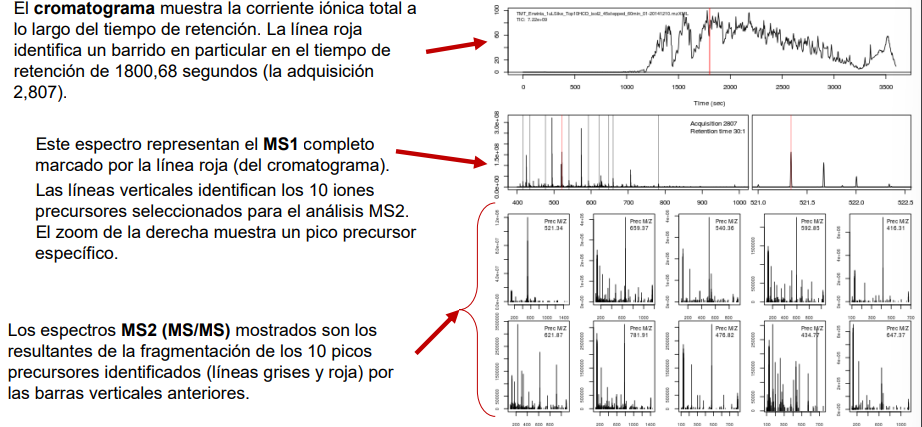
\includegraphics[width = \textwidth]{figs/espectro-analisis.png}
\caption{La figura superior indica el cromatograma obtenido. Primero hay un tiempo de retención con la intensidad encontrada de toda la carga iónica recibidas. A partir de un tiempo de retención señalado con la línea roja, empieza el tiempo de adquisición. El MS1 (panel central) es la ampliación de la línea roja del cromatograma. Cada línea vertical indica la masa detectada con sus intensidades. La parte derecha es un zoom de la línea roja. El MS1 se genera por cada péptido encontrado. Para este ejemplo, se cogen los iones marcados en gris y rojo y se fragmentan. Se saca la masa, carga e intensidad por cada uno de los iones en el segundo analizador. }
\end{figure}

La siguiente imagen muestra una representación de un LC-MS. A partir de un determinado tiempo de retención, hay una serie de masas cargas de los péptidos con una intensidad asociada a cada uno. Para diferentes tiempos de retención hay diferentes picos del espectrómetro.

\begin{figure}[h]
\centering
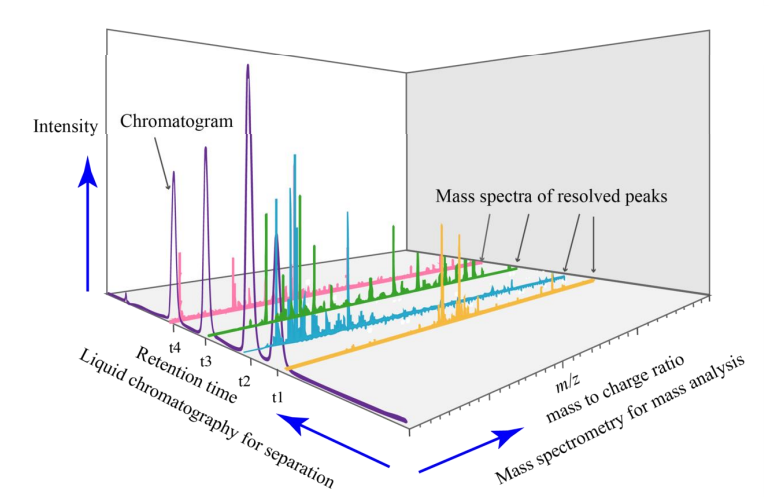
\includegraphics[width = \textwidth]{figs/lc-ms.png}
\end{figure}

Se tienden a coger los picos con mayor intensidad, ya que el resto son ruido del espectrómetro. Se sabe que a la hora de tener los péptidos, hay unos iones que van del extremo N-terminal al C-terminal y otros que van en sentido contrario. Estos iones van calculando la masa acumulativa. De esta forma se pueden saber los aminoácidos que componen el espectro.

\begin{figure}[h]
\centering
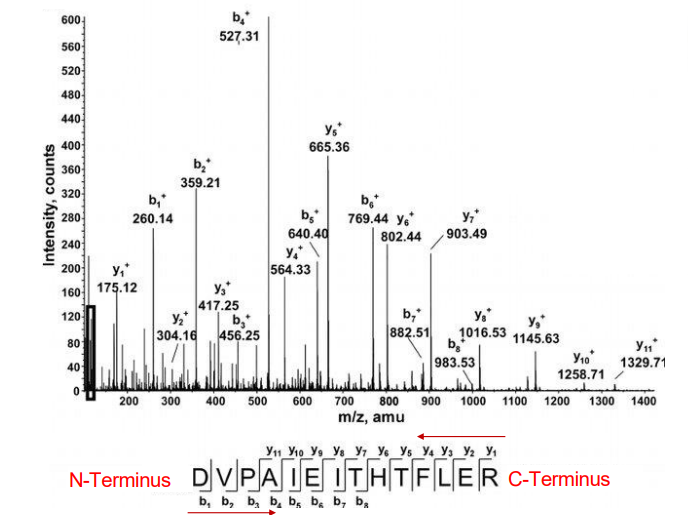
\includegraphics[width = 0.6\textwidth]{figs/fragmentacion-msms.png}
\end{figure}

\subsection{Adquisición de datos}
La adquisición de datos en espectrometría de masas puede realizarse de dos formas principales:
\begin{itemize}
\item \textbf{Adquisición dependiente de datos (DDA)}: En este modo, los iones más abundantes detectados en el espectro MS1 se seleccionan para su fragmentación, generando espectros MS2. Este proceso se repite secuencialmente para múltiples iones.
\item \textbf{Adquisición independiente de datos (DIA)}: En este modo, se fragmentan regiones específicas del espectro MS1, independientemente de la intensidad de los iones. Esto permite la detección de iones de baja abundancia, aunque puede resultar en espectros MS2 más complejos debido a la co-fragmentación de múltiples péptidos.
\end{itemize}

\begin{figure}[h]
\centering
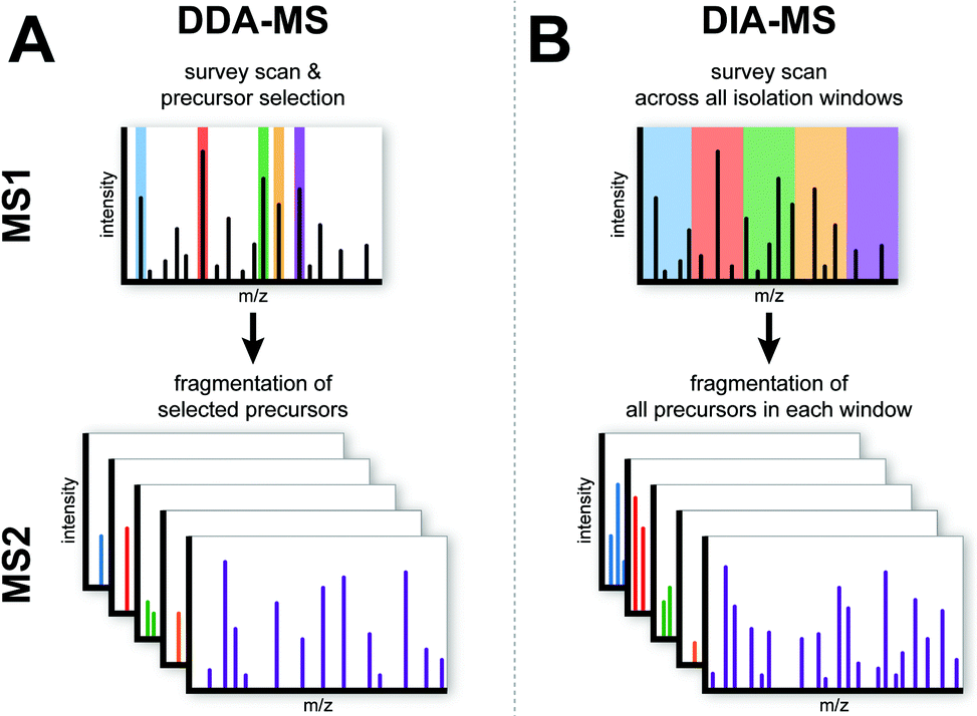
\includegraphics[width = 0.6\textwidth]{figs/data-adquisition.png}
\end{figure}

\subsection{Identificación de péptidos y proteínas}
La identificación de péptidos y proteínas se realiza comparando los espectros experimentales con bases de datos teóricas. Estas bases de datos contienen información sobre las masas y secuencias de péptidos generados in silico a partir de proteínas conocidas. Al comparar los espectros experimentales con los teóricos, se puede determinar la secuencia de aminoácidos de los péptidos y, por tanto, identificar las proteínas presentes en la muestra. Cada identificación se asocia con un score de confianza que indica la fiabilidad del resultado.

\subsection{Aplicaciones de la proteómica "Bottom-Up"}
La proteómica "Bottom-Up" tiene dos enfoques principales:
\begin{itemize}
\item \textbf{Proteómica de descubrimiento (Discovery Proteomics)}: Se utiliza para analizar proteomas completos, identificando y cuantificando proteínas de abundancia moderada a alta. Un posible ejemplo es la búsqueda de posibles biomarcadores.
\item \textbf{Proteómica dirigida (Targeted Proteomics)}: Se centra en la cuantificación de proteínas específicas, incluso en bajas abundancias. Una técnica común en este enfoque es el monitoreo de reacciones seleccionadas/múltiples (SRM/MRM), que utiliza tres analizadores de cuadrupolo para seleccionar y cuantificar péptidos específicos. Un ejemplo de aplicación es la validación de biomarcadores.
\end{itemize}

\subsubsection{Cuantificación y estándares internos}
En la cuantificación de proteínas, es crucial utilizar estándares internos para corregir variaciones en la ionización y la eficiencia de la cromatografía. Estos estándares son péptidos sintéticos con propiedades similares a los péptidos de interés, pero marcados con isótopos estables. Al comparar las áreas bajo la curva de los péptidos de interés con las de los estándares internos, se obtiene una cuantificación precisa y reproducible.

\begin{figure}[h]
\centering
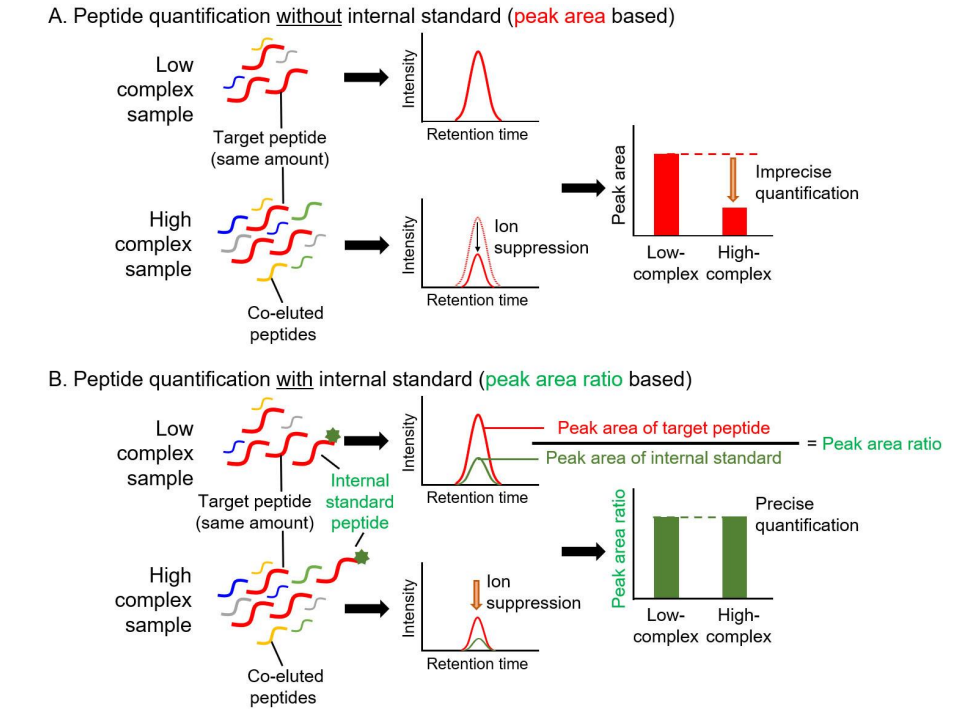
\includegraphics[width = 0.6\textwidth]{figs/internal-standard.png}
\end{figure}

%Cuando la muestra es compleja, los péptidos pueden competir causando colución. La intensidad va a disminuir al haber menos iones que se cuantificarán. La cuantificación de una muestra compleja será por tanto menor que el mismo péptido en una muestra poco compleja. Por esto, se establecen estándares internos: péptides con cualidades similares marcados. Se conoce la cantidad a priori del péptido asociado. Así, da igual si la complejidad es mucha o poca, ya que se establece la relación entre el péptido asociado y el péptido buscado. Lo que se calcula es el ratio del pico, es decir, el área del péptido buscado con el área del estándar interno. 

%\section{Proteómica "Top-Down"}

\section{FragPipe}
FragPipe es un software que engloba varios programas. El buscador es MSFragger, pero cuenta también con otras herramientas como Philosopher, PTM-Shepher, etc. Lo descargamos de GitHub y descargamos las licencias de MSFragger, IonQuant y diaTracer. 